% Latex template: mahmoud.s.fahmy@students.kasralainy.edu.eg
% For more details: https://www.sharelatex.com/learn/Beamer

\documentclass{beamer}					  % Document class

\usepackage[portuguese]{babel}			  % Set language
\usepackage[utf8x]{inputenc}			  % Set encoding

\mode<presentation> {					  % Set options
  \usetheme{default}					    % Set theme
  \usecolortheme{default} 				% Set colors
  \usefonttheme{default}  				% Set font theme
  \setbeamertemplate{caption}[numbered]	% Set caption to be numbered
}

\setbeamertemplate{navigation symbols}{}
\setbeamertemplate{footline}[frame number]
\setbeamercovered{transparent}

% Uncomment this to have the outline at the beginning of each section highlighted.
%\AtBeginSection[]
%{
%  \begin{frame}{Outline}
%    \tableofcontents[currentsection]
%  \end{frame}
%}

\usepackage{graphicx}					% For including figures
\usepackage{booktabs}					% For table rules
\usepackage{hyperref}					% For cross-referencing
\usepackage{caption}                    % Allows more control over captions in figs and tables

\title{Revisão de Atividades da FAC}	% Presentation title
%\author{Author One}					% Presentation author
\institute{LNLS.DAC.FAC}				% Author affiliation
\date{2024-02-16 -- 2024-03-08}			% Today's date	


\begin{document}



\begin{frame}
  \titlepage
  \href{https://github.com/lnls-fac/doc-review-dac-fac}{\beamergotobutton{Link para o repo github desta apresentação: https://github.com/lnls-fac/doc-review-dac-fac}}
  \href{https://www.overleaf.com/read/sbdjxtzfchrm}{\beamergotobutton{Link para o projeto overleaf destas notas}}
\end{frame}

\begin{frame}{Outline}
  \tableofcontents
\end{frame}




% \section{CBI Transversais}

% \begin{frame}{CBI Transversais}
%     \scriptsize{\begin{itemize}
%             \item Estudo de máquina 29/01, BbB
%     \end{itemize}}
%     \begin{figure}[H]
%         	\centering
%             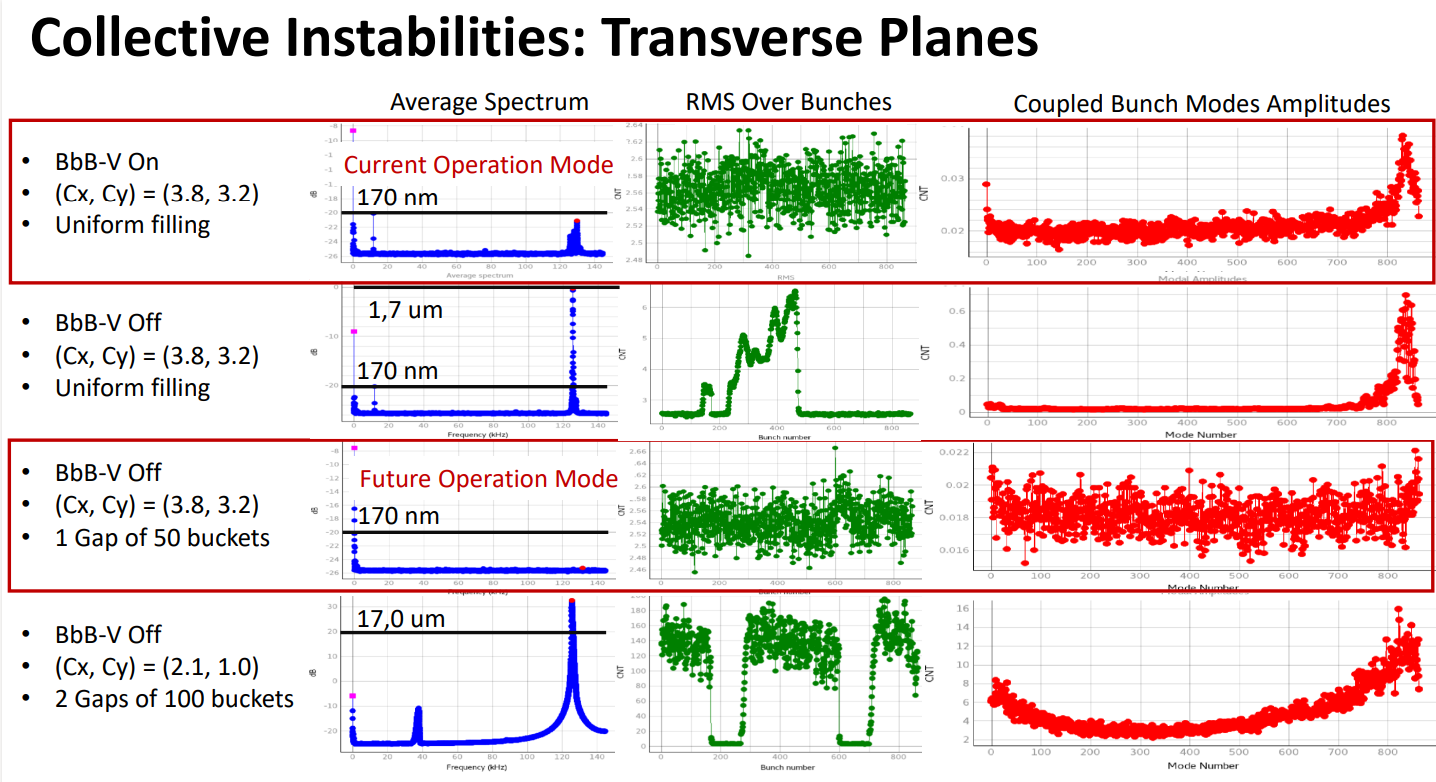
\includegraphics[width=1.0\textwidth]{2024-03-08/figures/cbi-transversais.png}
%             \label{fig:cbi-transversal}
%     \end{figure} 
% \end{frame}



\section{NLK}

\begin{frame}{NLK}
    Experimento:
    \begin{itemize}
    		\item Pulso H full-sine: otimização iterativa (delay, amp) $\rightarrow$ ficou pior que com pulso half-sine.
            \item Retorno da eletrônica anterior das bobinas compensadoras
            \item Re-otimização: H,V delays = (380, 0)*8 ns; H,V amps = (131, 65) V
    \end{itemize}
    \begin{figure}[H]
      \centering
          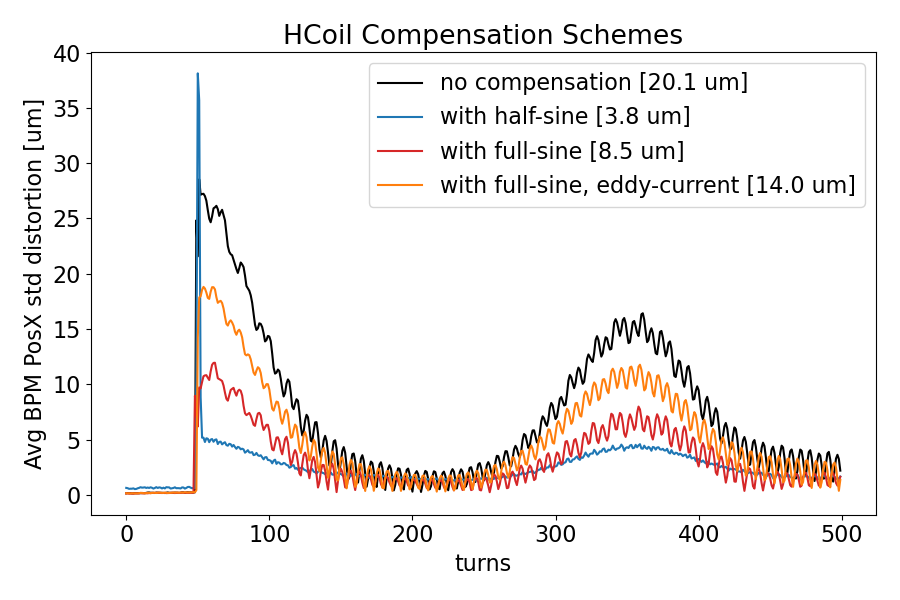
\includegraphics[width=1\textwidth]{2024-03-08/figures/hcoil-compensation-scheme.png}
          \label{fig:hcoil-scheme}
    \end{figure}
\end{frame}



\section{Ótica do Booster}

\begin{frame}{Ótica do Booster}
    \begin{figure}[H]
    		\centering
            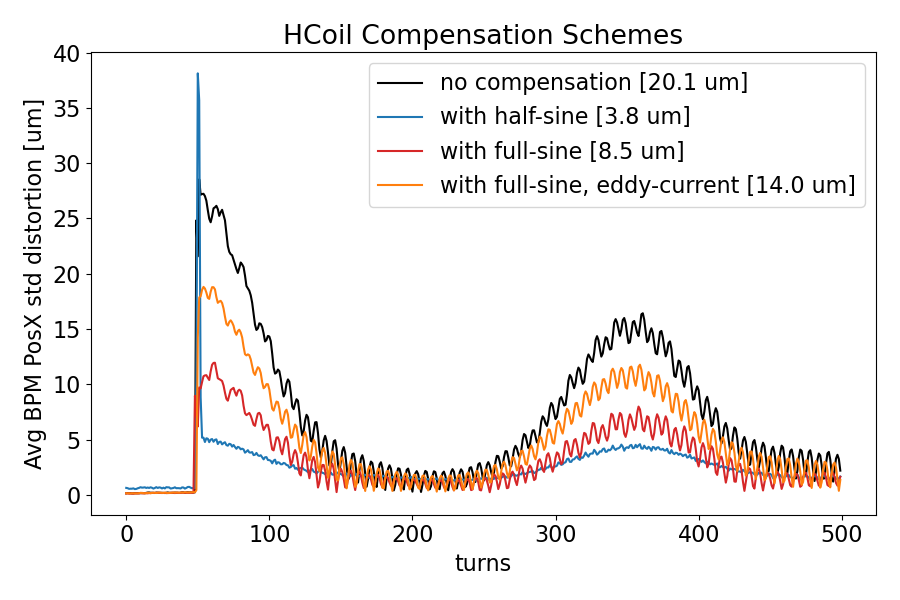
\includegraphics[width=1.1\textwidth]{2024-03-08/figures/hcoil-compensation-scheme.png}
            \label{fig:bo-ramp}
    \end{figure}
\end{frame}



\section{References}



\end{document}
